%================================================
% FLUXOGRAMA MESTRE DO LIVRO
%================================================
\cleardoublepage

\chapter*{Fluxograma Mestre}
\addcontentsline{toc}{chapter}{Fluxograma Mestre da Modelagem de Distribuição de Espécies}

\section*{Visão geral}

A Modelagem de Distribuição de Espécies (\textit{Species Distribution Modeling} -- SDM)
constitui uma estrutura integrada de inferência ecológica que combina
biogeografia, ecologia, climatologia, ciência de dados espaciais e modelagem
estatística para compreender e projetar a distribuição das espécies no espaço
e no tempo.

Embora frequentemente apresentada como uma sequência de algoritmos
computacionais, a SDM é fundamentalmente uma abordagem ecológica baseada na
relação entre organismos e ambiente. Cada etapa do processo influencia
diretamente a qualidade dos modelos, a interpretação dos resultados e a
robustez das inferências produzidas.

O fluxograma apresentado na Figura~\ref{fig:fluxograma-mestre-sdm}
resume o fluxo de trabalho adotado neste livro, desde a teoria ecológica
do nicho até aplicações em conservação da biodiversidade sob cenários de
mudanças climáticas.

\begin{figure}[p]
	\centering
	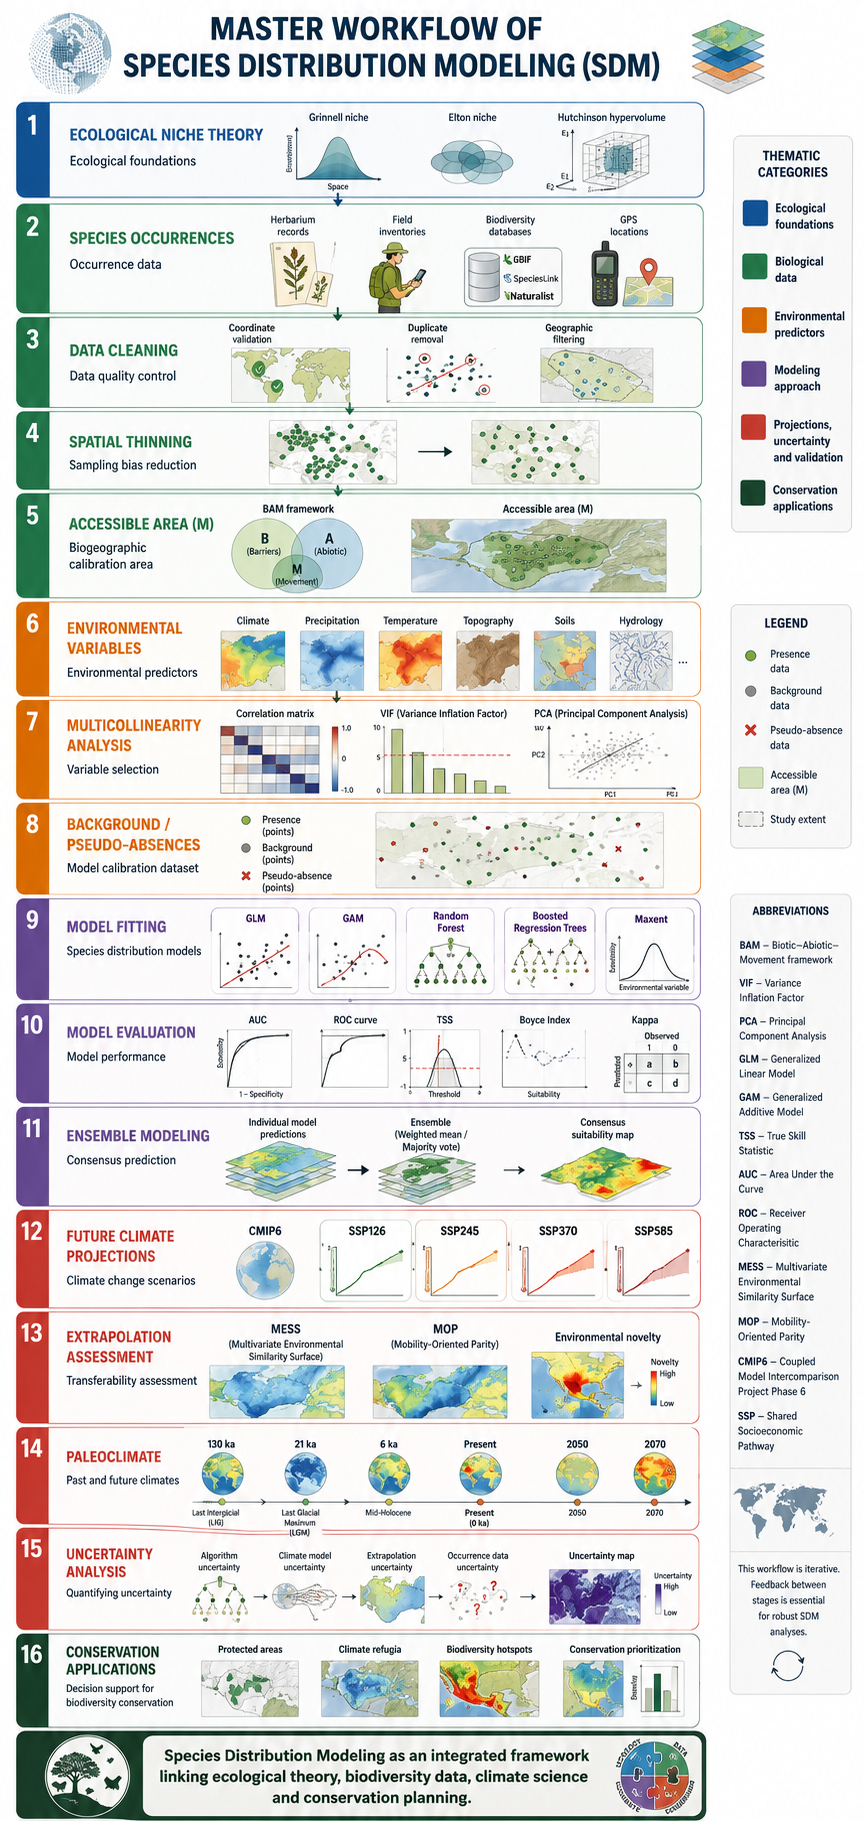
\includegraphics[
	width=0.95\textwidth,
	height=0.88\textheight,
	keepaspectratio
	]{figuras/fluxograma_mestre_sdm.png}
	
	\caption{
		Fluxograma mestre da Modelagem de Distribuição de Espécies (SDM)
		utilizado neste livro. O fluxo integra fundamentos ecológicos,
		dados de ocorrência, limpeza e rarefação espacial, definição da área acessível
		($M$), variáveis ambientais, multicolinearidade, background e pseudo-ausências,
		ajuste e avaliação de modelos, modelagem ensemble, projeções climáticas futuras,
		paleoclima, extrapolação, quantificação de incertezas e aplicações em conservação
		da biodiversidade. As cores representam grandes componentes conceituais do
		processo: fundamentos ecológicos, dados biológicos, preditores ambientais,
		modelagem, projeções climáticas, incertezas e aplicações em conservação.
	}
	\label{fig:fluxograma-mestre-sdm}
\end{figure}

\cleardoublepage

\section*{Como interpretar o fluxograma}

O processo inicia-se com a teoria ecológica do nicho, que fornece a base
conceitual para compreender a distribuição das espécies em função de gradientes
ambientais. Em seguida, registros de ocorrência são obtidos, validados e
submetidos a procedimentos de limpeza e rarefação espacial para reduzir erros
e vieses amostrais.

Posteriormente, define-se a área acessível ($M$) da espécie, conforme o
\textit{BAM framework}, e selecionam-se variáveis ambientais potencialmente
relevantes para explicar sua distribuição. Essas variáveis devem ser avaliadas
quanto à multicolinearidade por meio de correlação, VIF e outras abordagens de
seleção.

Após a construção da base de modelagem, são gerados pontos de background ou
pseudo-ausências e ajustados diferentes algoritmos, incluindo GLM, GAM,
Random Forest, Boosted Regression Trees e Maxent. Os modelos resultantes são
avaliados por métricas de desempenho e posteriormente integrados em modelos
ensemble.

Os modelos calibrados podem então ser projetados para cenários climáticos
futuros, períodos paleoclimáticos ou novas regiões geográficas. Nessas
situações, torna-se essencial avaliar a extrapolação ambiental utilizando
ferramentas como MESS e MOP.

Finalmente, diferentes fontes de incerteza são quantificadas e incorporadas
às análises, permitindo aplicações robustas em conservação, planejamento
ambiental, identificação de refúgios climáticos e priorização de áreas para
proteção da biodiversidade.

\begin{center}
	\fbox{
		\begin{minipage}{0.90\textwidth}
			
			\textbf{Síntese metodológica.}
			
			A qualidade de um modelo de distribuição não depende exclusivamente do
			algoritmo utilizado. Em muitos estudos, decisões tomadas durante a preparação
			dos dados, seleção de variáveis, definição da área acessível ($M$) e avaliação
			da extrapolação exercem impacto maior sobre os resultados finais do que a
			escolha do algoritmo propriamente dita.
			
		\end{minipage}
	}
\end{center}

\section*{Relação entre o fluxograma e as unidades do livro}

\begin{table}[H]
	\centering
	\caption{Correspondência entre as etapas do fluxo de trabalho e as unidades do livro.}
	\begin{tabular}{ll}
		\toprule
		Etapa do fluxograma & Unidade correspondente \\
		\midrule
		Teoria ecológica do nicho & Unidade 1 \\
		Ocorrências, limpeza e rarefação espacial & Unidade 2 \\
		Variáveis ambientais & Unidade 3 \\
		Multicolinearidade & Unidade 4 \\
		Área acessível ($M$) & Unidade 5 \\
		GLM & Unidade 6 \\
		GAM & Unidade 7 \\
		Random Forest & Unidade 8 \\
		BRT & Unidade 9 \\
		Maxent & Unidade 10 \\
		Ensemble & Unidade 11 \\
		Avaliação de modelos & Unidade 12 \\
		Projeções climáticas futuras & Unidade 13 \\
		Transferência e extrapolação & Unidade 14 \\
		Paleoclima & Unidade 15 \\
		Incertezas em SDM & Unidade 16 \\
		Aplicações à conservação & Unidade 17 \\
		Considerações finais & Unidade 18 \\
		\bottomrule
	\end{tabular}
\end{table}

\clearpage
